\documentclass{beamer}
\usetheme{Boadilla}
\usecolortheme{whale}

\usepackage{wrapfig}
\usepackage{pgf}

\newcommand{\includepgf}[3]{\resizebox{#1}{#2}{\input{#3}}}

\AtBeginSection[]{
  \begin{frame}
  \vfill
  \centering
  \begin{beamercolorbox}[sep=8pt,center,shadow=true,rounded=true]{title}
    \usebeamerfont{title}\insertsectionhead\par%
  \end{beamercolorbox}
  \vfill
  \end{frame}
}

\title[MSc Thesis 2]
{Second MSc thesis presentation}


\author[V. BARBAZA]{Valentin BARBAZA}

\date[2023] % (optional)
{May 2023}

\logo{
\includegraphics[height=0.7cm]{figures/istnewlogo.pdf}}

\definecolor{istblue}{RGB}{0,102,153}
\setbeamercolor{titlelike}{bg=istblue}
\setbeamerfont{title}{series=\bfseries}

\begin{document}

\frame{\titlepage}

\begin{frame}
\frametitle{Table of Contents}
\tableofcontents
\end{frame}

\section{Sub circuits}
\subsection{Activation functions}

\begin{frame}
\frametitle{Sigmoid}
I reproduced the sigmoid circuit described in the base paper, adjusted the parameters to optain the following results :
\begin{figure}
    \centering
      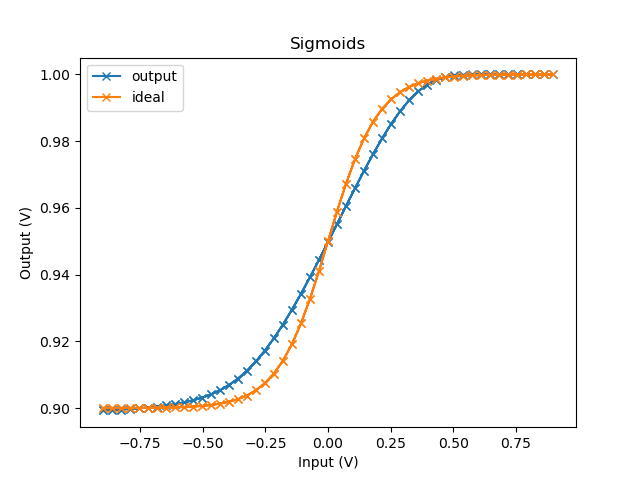
\includegraphics[height=0.5\textheight]{figures/sigmoid.png}
\end{figure}
\end{frame}

\begin{frame}
\frametitle{Hyperbolic Tangent}
The second activation function used is the tanh function. Using the same circuit with a slight change in the parameters we get the following :
\begin{figure}    
    \centering
    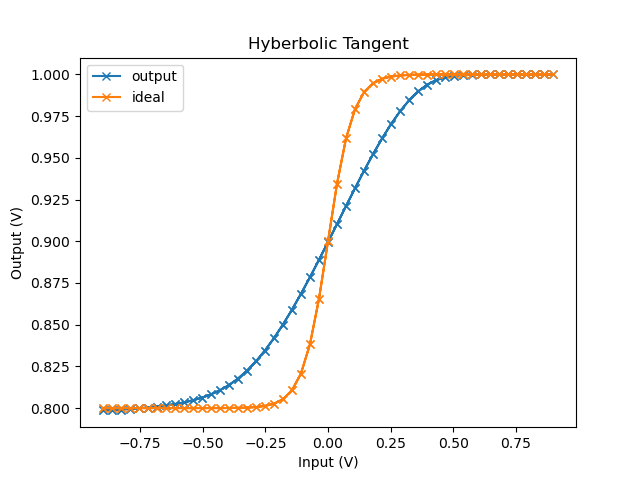
\includegraphics[height=0.5\textheight]{figures/tanh.png}
\end{figure}
They both use ideal verilog-A model for their OpAmp
\end{frame}

\subsection{Memory cells}
\begin{frame}{The memory cell}
    In order to store an analog value until the next LSTM step.
    \begin{figure}    
        \centering
        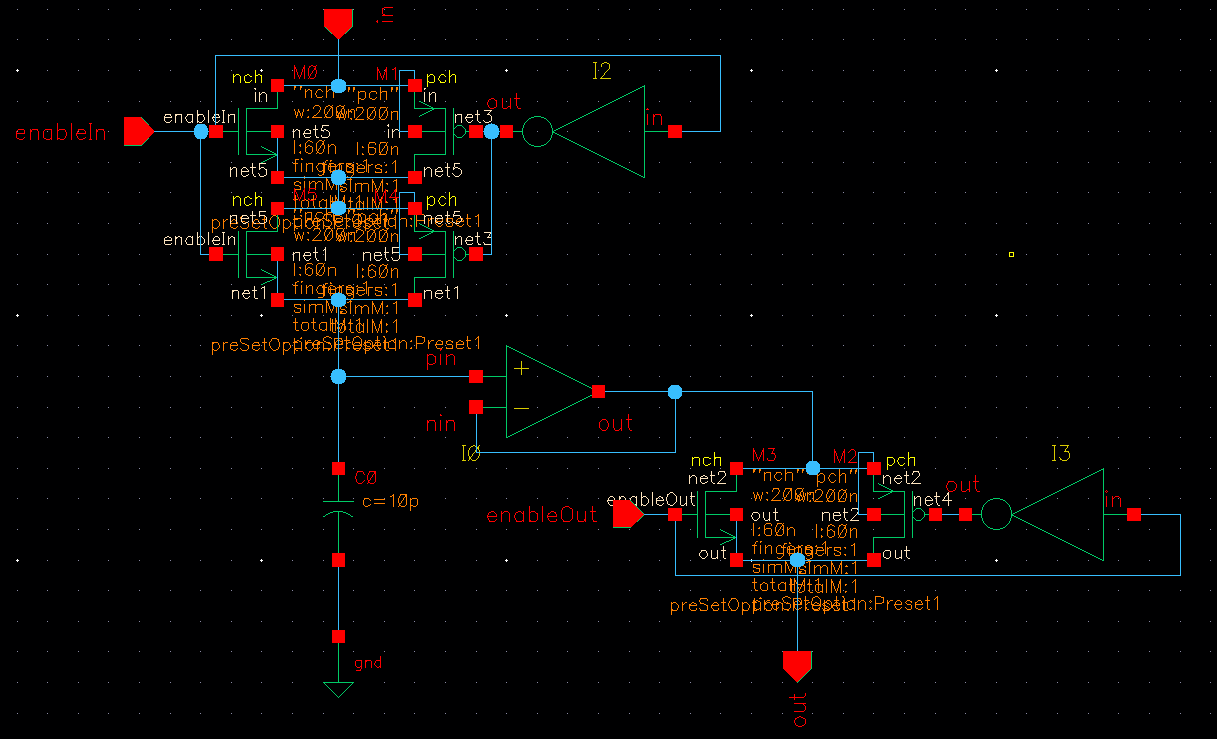
\includegraphics[height=0.5\textheight]{figures/memcell-circuit.png}
    \end{figure}
    The memory cell has 2 CMOS switches to avoid the memory to be influenced by the voltage in the input.
\end{frame}
\begin{frame}{Memory leaks}
    Here is the value stored in the unit over time with one and two CMOS switches.
    \begin{figure}
        \centering
        \resizebox{!}{0.4\textheight}{%% Creator: Matplotlib, PGF backend
%%
%% To include the figure in your LaTeX document, write
%%   \input{<filename>.pgf}
%%
%% Make sure the required packages are loaded in your preamble
%%   \usepackage{pgf}
%%
%% Also ensure that all the required font packages are loaded; for instance,
%% the lmodern package is sometimes necessary when using math font.
%%   \usepackage{lmodern}
%%
%% Figures using additional raster images can only be included by \input if
%% they are in the same directory as the main LaTeX file. For loading figures
%% from other directories you can use the `import` package
%%   \usepackage{import}
%%
%% and then include the figures with
%%   \import{<path to file>}{<filename>.pgf}
%%
%% Matplotlib used the following preamble
%%   
%%   \usepackage{fontspec}
%%   \setmainfont{DejaVuSerif.ttf}[Path=\detokenize{/usr/lib/python3.11/site-packages/matplotlib/mpl-data/fonts/ttf/}]
%%   \setsansfont{DejaVuSans.ttf}[Path=\detokenize{/usr/lib/python3.11/site-packages/matplotlib/mpl-data/fonts/ttf/}]
%%   \setmonofont{DejaVuSansMono.ttf}[Path=\detokenize{/usr/lib/python3.11/site-packages/matplotlib/mpl-data/fonts/ttf/}]
%%   \makeatletter\@ifpackageloaded{underscore}{}{\usepackage[strings]{underscore}}\makeatother
%%
\begingroup%
\makeatletter%
\begin{pgfpicture}%
\pgfpathrectangle{\pgfpointorigin}{\pgfqpoint{6.400000in}{4.800000in}}%
\pgfusepath{use as bounding box, clip}%
\begin{pgfscope}%
\pgfsetbuttcap%
\pgfsetmiterjoin%
\definecolor{currentfill}{rgb}{1.000000,1.000000,1.000000}%
\pgfsetfillcolor{currentfill}%
\pgfsetlinewidth{0.000000pt}%
\definecolor{currentstroke}{rgb}{1.000000,1.000000,1.000000}%
\pgfsetstrokecolor{currentstroke}%
\pgfsetdash{}{0pt}%
\pgfpathmoveto{\pgfqpoint{0.000000in}{0.000000in}}%
\pgfpathlineto{\pgfqpoint{6.400000in}{0.000000in}}%
\pgfpathlineto{\pgfqpoint{6.400000in}{4.800000in}}%
\pgfpathlineto{\pgfqpoint{0.000000in}{4.800000in}}%
\pgfpathlineto{\pgfqpoint{0.000000in}{0.000000in}}%
\pgfpathclose%
\pgfusepath{fill}%
\end{pgfscope}%
\begin{pgfscope}%
\pgfsetbuttcap%
\pgfsetmiterjoin%
\definecolor{currentfill}{rgb}{1.000000,1.000000,1.000000}%
\pgfsetfillcolor{currentfill}%
\pgfsetlinewidth{0.000000pt}%
\definecolor{currentstroke}{rgb}{0.000000,0.000000,0.000000}%
\pgfsetstrokecolor{currentstroke}%
\pgfsetstrokeopacity{0.000000}%
\pgfsetdash{}{0pt}%
\pgfpathmoveto{\pgfqpoint{0.800000in}{0.528000in}}%
\pgfpathlineto{\pgfqpoint{5.760000in}{0.528000in}}%
\pgfpathlineto{\pgfqpoint{5.760000in}{4.224000in}}%
\pgfpathlineto{\pgfqpoint{0.800000in}{4.224000in}}%
\pgfpathlineto{\pgfqpoint{0.800000in}{0.528000in}}%
\pgfpathclose%
\pgfusepath{fill}%
\end{pgfscope}%
\begin{pgfscope}%
\pgfsetbuttcap%
\pgfsetroundjoin%
\definecolor{currentfill}{rgb}{0.000000,0.000000,0.000000}%
\pgfsetfillcolor{currentfill}%
\pgfsetlinewidth{0.803000pt}%
\definecolor{currentstroke}{rgb}{0.000000,0.000000,0.000000}%
\pgfsetstrokecolor{currentstroke}%
\pgfsetdash{}{0pt}%
\pgfsys@defobject{currentmarker}{\pgfqpoint{0.000000in}{-0.048611in}}{\pgfqpoint{0.000000in}{0.000000in}}{%
\pgfpathmoveto{\pgfqpoint{0.000000in}{0.000000in}}%
\pgfpathlineto{\pgfqpoint{0.000000in}{-0.048611in}}%
\pgfusepath{stroke,fill}%
}%
\begin{pgfscope}%
\pgfsys@transformshift{1.017927in}{0.528000in}%
\pgfsys@useobject{currentmarker}{}%
\end{pgfscope}%
\end{pgfscope}%
\begin{pgfscope}%
\definecolor{textcolor}{rgb}{0.000000,0.000000,0.000000}%
\pgfsetstrokecolor{textcolor}%
\pgfsetfillcolor{textcolor}%
\pgftext[x=1.017927in,y=0.430778in,,top]{\color{textcolor}\sffamily\fontsize{10.000000}{12.000000}\selectfont 0}%
\end{pgfscope}%
\begin{pgfscope}%
\pgfsetbuttcap%
\pgfsetroundjoin%
\definecolor{currentfill}{rgb}{0.000000,0.000000,0.000000}%
\pgfsetfillcolor{currentfill}%
\pgfsetlinewidth{0.803000pt}%
\definecolor{currentstroke}{rgb}{0.000000,0.000000,0.000000}%
\pgfsetstrokecolor{currentstroke}%
\pgfsetdash{}{0pt}%
\pgfsys@defobject{currentmarker}{\pgfqpoint{0.000000in}{-0.048611in}}{\pgfqpoint{0.000000in}{0.000000in}}{%
\pgfpathmoveto{\pgfqpoint{0.000000in}{0.000000in}}%
\pgfpathlineto{\pgfqpoint{0.000000in}{-0.048611in}}%
\pgfusepath{stroke,fill}%
}%
\begin{pgfscope}%
\pgfsys@transformshift{1.770697in}{0.528000in}%
\pgfsys@useobject{currentmarker}{}%
\end{pgfscope}%
\end{pgfscope}%
\begin{pgfscope}%
\definecolor{textcolor}{rgb}{0.000000,0.000000,0.000000}%
\pgfsetstrokecolor{textcolor}%
\pgfsetfillcolor{textcolor}%
\pgftext[x=1.770697in,y=0.430778in,,top]{\color{textcolor}\sffamily\fontsize{10.000000}{12.000000}\selectfont 20}%
\end{pgfscope}%
\begin{pgfscope}%
\pgfsetbuttcap%
\pgfsetroundjoin%
\definecolor{currentfill}{rgb}{0.000000,0.000000,0.000000}%
\pgfsetfillcolor{currentfill}%
\pgfsetlinewidth{0.803000pt}%
\definecolor{currentstroke}{rgb}{0.000000,0.000000,0.000000}%
\pgfsetstrokecolor{currentstroke}%
\pgfsetdash{}{0pt}%
\pgfsys@defobject{currentmarker}{\pgfqpoint{0.000000in}{-0.048611in}}{\pgfqpoint{0.000000in}{0.000000in}}{%
\pgfpathmoveto{\pgfqpoint{0.000000in}{0.000000in}}%
\pgfpathlineto{\pgfqpoint{0.000000in}{-0.048611in}}%
\pgfusepath{stroke,fill}%
}%
\begin{pgfscope}%
\pgfsys@transformshift{2.523466in}{0.528000in}%
\pgfsys@useobject{currentmarker}{}%
\end{pgfscope}%
\end{pgfscope}%
\begin{pgfscope}%
\definecolor{textcolor}{rgb}{0.000000,0.000000,0.000000}%
\pgfsetstrokecolor{textcolor}%
\pgfsetfillcolor{textcolor}%
\pgftext[x=2.523466in,y=0.430778in,,top]{\color{textcolor}\sffamily\fontsize{10.000000}{12.000000}\selectfont 40}%
\end{pgfscope}%
\begin{pgfscope}%
\pgfsetbuttcap%
\pgfsetroundjoin%
\definecolor{currentfill}{rgb}{0.000000,0.000000,0.000000}%
\pgfsetfillcolor{currentfill}%
\pgfsetlinewidth{0.803000pt}%
\definecolor{currentstroke}{rgb}{0.000000,0.000000,0.000000}%
\pgfsetstrokecolor{currentstroke}%
\pgfsetdash{}{0pt}%
\pgfsys@defobject{currentmarker}{\pgfqpoint{0.000000in}{-0.048611in}}{\pgfqpoint{0.000000in}{0.000000in}}{%
\pgfpathmoveto{\pgfqpoint{0.000000in}{0.000000in}}%
\pgfpathlineto{\pgfqpoint{0.000000in}{-0.048611in}}%
\pgfusepath{stroke,fill}%
}%
\begin{pgfscope}%
\pgfsys@transformshift{3.276236in}{0.528000in}%
\pgfsys@useobject{currentmarker}{}%
\end{pgfscope}%
\end{pgfscope}%
\begin{pgfscope}%
\definecolor{textcolor}{rgb}{0.000000,0.000000,0.000000}%
\pgfsetstrokecolor{textcolor}%
\pgfsetfillcolor{textcolor}%
\pgftext[x=3.276236in,y=0.430778in,,top]{\color{textcolor}\sffamily\fontsize{10.000000}{12.000000}\selectfont 60}%
\end{pgfscope}%
\begin{pgfscope}%
\pgfsetbuttcap%
\pgfsetroundjoin%
\definecolor{currentfill}{rgb}{0.000000,0.000000,0.000000}%
\pgfsetfillcolor{currentfill}%
\pgfsetlinewidth{0.803000pt}%
\definecolor{currentstroke}{rgb}{0.000000,0.000000,0.000000}%
\pgfsetstrokecolor{currentstroke}%
\pgfsetdash{}{0pt}%
\pgfsys@defobject{currentmarker}{\pgfqpoint{0.000000in}{-0.048611in}}{\pgfqpoint{0.000000in}{0.000000in}}{%
\pgfpathmoveto{\pgfqpoint{0.000000in}{0.000000in}}%
\pgfpathlineto{\pgfqpoint{0.000000in}{-0.048611in}}%
\pgfusepath{stroke,fill}%
}%
\begin{pgfscope}%
\pgfsys@transformshift{4.029006in}{0.528000in}%
\pgfsys@useobject{currentmarker}{}%
\end{pgfscope}%
\end{pgfscope}%
\begin{pgfscope}%
\definecolor{textcolor}{rgb}{0.000000,0.000000,0.000000}%
\pgfsetstrokecolor{textcolor}%
\pgfsetfillcolor{textcolor}%
\pgftext[x=4.029006in,y=0.430778in,,top]{\color{textcolor}\sffamily\fontsize{10.000000}{12.000000}\selectfont 80}%
\end{pgfscope}%
\begin{pgfscope}%
\pgfsetbuttcap%
\pgfsetroundjoin%
\definecolor{currentfill}{rgb}{0.000000,0.000000,0.000000}%
\pgfsetfillcolor{currentfill}%
\pgfsetlinewidth{0.803000pt}%
\definecolor{currentstroke}{rgb}{0.000000,0.000000,0.000000}%
\pgfsetstrokecolor{currentstroke}%
\pgfsetdash{}{0pt}%
\pgfsys@defobject{currentmarker}{\pgfqpoint{0.000000in}{-0.048611in}}{\pgfqpoint{0.000000in}{0.000000in}}{%
\pgfpathmoveto{\pgfqpoint{0.000000in}{0.000000in}}%
\pgfpathlineto{\pgfqpoint{0.000000in}{-0.048611in}}%
\pgfusepath{stroke,fill}%
}%
\begin{pgfscope}%
\pgfsys@transformshift{4.781776in}{0.528000in}%
\pgfsys@useobject{currentmarker}{}%
\end{pgfscope}%
\end{pgfscope}%
\begin{pgfscope}%
\definecolor{textcolor}{rgb}{0.000000,0.000000,0.000000}%
\pgfsetstrokecolor{textcolor}%
\pgfsetfillcolor{textcolor}%
\pgftext[x=4.781776in,y=0.430778in,,top]{\color{textcolor}\sffamily\fontsize{10.000000}{12.000000}\selectfont 100}%
\end{pgfscope}%
\begin{pgfscope}%
\pgfsetbuttcap%
\pgfsetroundjoin%
\definecolor{currentfill}{rgb}{0.000000,0.000000,0.000000}%
\pgfsetfillcolor{currentfill}%
\pgfsetlinewidth{0.803000pt}%
\definecolor{currentstroke}{rgb}{0.000000,0.000000,0.000000}%
\pgfsetstrokecolor{currentstroke}%
\pgfsetdash{}{0pt}%
\pgfsys@defobject{currentmarker}{\pgfqpoint{0.000000in}{-0.048611in}}{\pgfqpoint{0.000000in}{0.000000in}}{%
\pgfpathmoveto{\pgfqpoint{0.000000in}{0.000000in}}%
\pgfpathlineto{\pgfqpoint{0.000000in}{-0.048611in}}%
\pgfusepath{stroke,fill}%
}%
\begin{pgfscope}%
\pgfsys@transformshift{5.534545in}{0.528000in}%
\pgfsys@useobject{currentmarker}{}%
\end{pgfscope}%
\end{pgfscope}%
\begin{pgfscope}%
\definecolor{textcolor}{rgb}{0.000000,0.000000,0.000000}%
\pgfsetstrokecolor{textcolor}%
\pgfsetfillcolor{textcolor}%
\pgftext[x=5.534545in,y=0.430778in,,top]{\color{textcolor}\sffamily\fontsize{10.000000}{12.000000}\selectfont 120}%
\end{pgfscope}%
\begin{pgfscope}%
\definecolor{textcolor}{rgb}{0.000000,0.000000,0.000000}%
\pgfsetstrokecolor{textcolor}%
\pgfsetfillcolor{textcolor}%
\pgftext[x=3.280000in,y=0.240809in,,top]{\color{textcolor}\sffamily\fontsize{10.000000}{12.000000}\selectfont Time (\(\displaystyle \mu s\))}%
\end{pgfscope}%
\begin{pgfscope}%
\pgfsetbuttcap%
\pgfsetroundjoin%
\definecolor{currentfill}{rgb}{0.000000,0.000000,0.000000}%
\pgfsetfillcolor{currentfill}%
\pgfsetlinewidth{0.803000pt}%
\definecolor{currentstroke}{rgb}{0.000000,0.000000,0.000000}%
\pgfsetstrokecolor{currentstroke}%
\pgfsetdash{}{0pt}%
\pgfsys@defobject{currentmarker}{\pgfqpoint{-0.048611in}{0.000000in}}{\pgfqpoint{-0.000000in}{0.000000in}}{%
\pgfpathmoveto{\pgfqpoint{-0.000000in}{0.000000in}}%
\pgfpathlineto{\pgfqpoint{-0.048611in}{0.000000in}}%
\pgfusepath{stroke,fill}%
}%
\begin{pgfscope}%
\pgfsys@transformshift{0.800000in}{0.574883in}%
\pgfsys@useobject{currentmarker}{}%
\end{pgfscope}%
\end{pgfscope}%
\begin{pgfscope}%
\definecolor{textcolor}{rgb}{0.000000,0.000000,0.000000}%
\pgfsetstrokecolor{textcolor}%
\pgfsetfillcolor{textcolor}%
\pgftext[x=0.481898in, y=0.522122in, left, base]{\color{textcolor}\sffamily\fontsize{10.000000}{12.000000}\selectfont 0.5}%
\end{pgfscope}%
\begin{pgfscope}%
\pgfsetbuttcap%
\pgfsetroundjoin%
\definecolor{currentfill}{rgb}{0.000000,0.000000,0.000000}%
\pgfsetfillcolor{currentfill}%
\pgfsetlinewidth{0.803000pt}%
\definecolor{currentstroke}{rgb}{0.000000,0.000000,0.000000}%
\pgfsetstrokecolor{currentstroke}%
\pgfsetdash{}{0pt}%
\pgfsys@defobject{currentmarker}{\pgfqpoint{-0.048611in}{0.000000in}}{\pgfqpoint{-0.000000in}{0.000000in}}{%
\pgfpathmoveto{\pgfqpoint{-0.000000in}{0.000000in}}%
\pgfpathlineto{\pgfqpoint{-0.048611in}{0.000000in}}%
\pgfusepath{stroke,fill}%
}%
\begin{pgfscope}%
\pgfsys@transformshift{0.800000in}{1.271095in}%
\pgfsys@useobject{currentmarker}{}%
\end{pgfscope}%
\end{pgfscope}%
\begin{pgfscope}%
\definecolor{textcolor}{rgb}{0.000000,0.000000,0.000000}%
\pgfsetstrokecolor{textcolor}%
\pgfsetfillcolor{textcolor}%
\pgftext[x=0.481898in, y=1.218334in, left, base]{\color{textcolor}\sffamily\fontsize{10.000000}{12.000000}\selectfont 0.6}%
\end{pgfscope}%
\begin{pgfscope}%
\pgfsetbuttcap%
\pgfsetroundjoin%
\definecolor{currentfill}{rgb}{0.000000,0.000000,0.000000}%
\pgfsetfillcolor{currentfill}%
\pgfsetlinewidth{0.803000pt}%
\definecolor{currentstroke}{rgb}{0.000000,0.000000,0.000000}%
\pgfsetstrokecolor{currentstroke}%
\pgfsetdash{}{0pt}%
\pgfsys@defobject{currentmarker}{\pgfqpoint{-0.048611in}{0.000000in}}{\pgfqpoint{-0.000000in}{0.000000in}}{%
\pgfpathmoveto{\pgfqpoint{-0.000000in}{0.000000in}}%
\pgfpathlineto{\pgfqpoint{-0.048611in}{0.000000in}}%
\pgfusepath{stroke,fill}%
}%
\begin{pgfscope}%
\pgfsys@transformshift{0.800000in}{1.967308in}%
\pgfsys@useobject{currentmarker}{}%
\end{pgfscope}%
\end{pgfscope}%
\begin{pgfscope}%
\definecolor{textcolor}{rgb}{0.000000,0.000000,0.000000}%
\pgfsetstrokecolor{textcolor}%
\pgfsetfillcolor{textcolor}%
\pgftext[x=0.481898in, y=1.914546in, left, base]{\color{textcolor}\sffamily\fontsize{10.000000}{12.000000}\selectfont 0.7}%
\end{pgfscope}%
\begin{pgfscope}%
\pgfsetbuttcap%
\pgfsetroundjoin%
\definecolor{currentfill}{rgb}{0.000000,0.000000,0.000000}%
\pgfsetfillcolor{currentfill}%
\pgfsetlinewidth{0.803000pt}%
\definecolor{currentstroke}{rgb}{0.000000,0.000000,0.000000}%
\pgfsetstrokecolor{currentstroke}%
\pgfsetdash{}{0pt}%
\pgfsys@defobject{currentmarker}{\pgfqpoint{-0.048611in}{0.000000in}}{\pgfqpoint{-0.000000in}{0.000000in}}{%
\pgfpathmoveto{\pgfqpoint{-0.000000in}{0.000000in}}%
\pgfpathlineto{\pgfqpoint{-0.048611in}{0.000000in}}%
\pgfusepath{stroke,fill}%
}%
\begin{pgfscope}%
\pgfsys@transformshift{0.800000in}{2.663520in}%
\pgfsys@useobject{currentmarker}{}%
\end{pgfscope}%
\end{pgfscope}%
\begin{pgfscope}%
\definecolor{textcolor}{rgb}{0.000000,0.000000,0.000000}%
\pgfsetstrokecolor{textcolor}%
\pgfsetfillcolor{textcolor}%
\pgftext[x=0.481898in, y=2.610758in, left, base]{\color{textcolor}\sffamily\fontsize{10.000000}{12.000000}\selectfont 0.8}%
\end{pgfscope}%
\begin{pgfscope}%
\pgfsetbuttcap%
\pgfsetroundjoin%
\definecolor{currentfill}{rgb}{0.000000,0.000000,0.000000}%
\pgfsetfillcolor{currentfill}%
\pgfsetlinewidth{0.803000pt}%
\definecolor{currentstroke}{rgb}{0.000000,0.000000,0.000000}%
\pgfsetstrokecolor{currentstroke}%
\pgfsetdash{}{0pt}%
\pgfsys@defobject{currentmarker}{\pgfqpoint{-0.048611in}{0.000000in}}{\pgfqpoint{-0.000000in}{0.000000in}}{%
\pgfpathmoveto{\pgfqpoint{-0.000000in}{0.000000in}}%
\pgfpathlineto{\pgfqpoint{-0.048611in}{0.000000in}}%
\pgfusepath{stroke,fill}%
}%
\begin{pgfscope}%
\pgfsys@transformshift{0.800000in}{3.359732in}%
\pgfsys@useobject{currentmarker}{}%
\end{pgfscope}%
\end{pgfscope}%
\begin{pgfscope}%
\definecolor{textcolor}{rgb}{0.000000,0.000000,0.000000}%
\pgfsetstrokecolor{textcolor}%
\pgfsetfillcolor{textcolor}%
\pgftext[x=0.481898in, y=3.306971in, left, base]{\color{textcolor}\sffamily\fontsize{10.000000}{12.000000}\selectfont 0.9}%
\end{pgfscope}%
\begin{pgfscope}%
\pgfsetbuttcap%
\pgfsetroundjoin%
\definecolor{currentfill}{rgb}{0.000000,0.000000,0.000000}%
\pgfsetfillcolor{currentfill}%
\pgfsetlinewidth{0.803000pt}%
\definecolor{currentstroke}{rgb}{0.000000,0.000000,0.000000}%
\pgfsetstrokecolor{currentstroke}%
\pgfsetdash{}{0pt}%
\pgfsys@defobject{currentmarker}{\pgfqpoint{-0.048611in}{0.000000in}}{\pgfqpoint{-0.000000in}{0.000000in}}{%
\pgfpathmoveto{\pgfqpoint{-0.000000in}{0.000000in}}%
\pgfpathlineto{\pgfqpoint{-0.048611in}{0.000000in}}%
\pgfusepath{stroke,fill}%
}%
\begin{pgfscope}%
\pgfsys@transformshift{0.800000in}{4.055944in}%
\pgfsys@useobject{currentmarker}{}%
\end{pgfscope}%
\end{pgfscope}%
\begin{pgfscope}%
\definecolor{textcolor}{rgb}{0.000000,0.000000,0.000000}%
\pgfsetstrokecolor{textcolor}%
\pgfsetfillcolor{textcolor}%
\pgftext[x=0.481898in, y=4.003183in, left, base]{\color{textcolor}\sffamily\fontsize{10.000000}{12.000000}\selectfont 1.0}%
\end{pgfscope}%
\begin{pgfscope}%
\definecolor{textcolor}{rgb}{0.000000,0.000000,0.000000}%
\pgfsetstrokecolor{textcolor}%
\pgfsetfillcolor{textcolor}%
\pgftext[x=0.426343in,y=2.376000in,,bottom,rotate=90.000000]{\color{textcolor}\sffamily\fontsize{10.000000}{12.000000}\selectfont Memory (V)}%
\end{pgfscope}%
\begin{pgfscope}%
\pgfpathrectangle{\pgfqpoint{0.800000in}{0.528000in}}{\pgfqpoint{4.960000in}{3.696000in}}%
\pgfusepath{clip}%
\pgfsetrectcap%
\pgfsetroundjoin%
\pgfsetlinewidth{1.505625pt}%
\definecolor{currentstroke}{rgb}{0.121569,0.466667,0.705882}%
\pgfsetstrokecolor{currentstroke}%
\pgfsetdash{}{0pt}%
\pgfpathmoveto{\pgfqpoint{1.025455in}{4.055836in}}%
\pgfpathlineto{\pgfqpoint{1.027336in}{4.055372in}}%
\pgfpathlineto{\pgfqpoint{1.029596in}{4.054480in}}%
\pgfpathlineto{\pgfqpoint{1.030442in}{4.046818in}}%
\pgfpathlineto{\pgfqpoint{1.030760in}{4.031162in}}%
\pgfpathlineto{\pgfqpoint{1.031395in}{3.809564in}}%
\pgfpathlineto{\pgfqpoint{1.031973in}{3.354234in}}%
\pgfpathlineto{\pgfqpoint{1.032099in}{3.234381in}}%
\pgfpathlineto{\pgfqpoint{1.032352in}{2.998289in}}%
\pgfpathlineto{\pgfqpoint{1.032667in}{2.706007in}}%
\pgfpathlineto{\pgfqpoint{1.032982in}{2.414210in}}%
\pgfpathlineto{\pgfqpoint{1.033140in}{2.325249in}}%
\pgfpathlineto{\pgfqpoint{1.033370in}{2.223545in}}%
\pgfpathlineto{\pgfqpoint{1.033591in}{2.162730in}}%
\pgfpathlineto{\pgfqpoint{1.034033in}{2.080062in}}%
\pgfpathlineto{\pgfqpoint{1.034516in}{2.020056in}}%
\pgfpathlineto{\pgfqpoint{1.035326in}{1.949643in}}%
\pgfpathlineto{\pgfqpoint{1.036430in}{1.883943in}}%
\pgfpathlineto{\pgfqpoint{1.038137in}{1.814018in}}%
\pgfpathlineto{\pgfqpoint{1.040551in}{1.746534in}}%
\pgfpathlineto{\pgfqpoint{1.044125in}{1.677927in}}%
\pgfpathlineto{\pgfqpoint{1.049282in}{1.610050in}}%
\pgfpathlineto{\pgfqpoint{1.056857in}{1.541579in}}%
\pgfpathlineto{\pgfqpoint{1.067870in}{1.473269in}}%
\pgfpathlineto{\pgfqpoint{1.083971in}{1.404684in}}%
\pgfpathlineto{\pgfqpoint{1.107424in}{1.336043in}}%
\pgfpathlineto{\pgfqpoint{1.141660in}{1.267128in}}%
\pgfpathlineto{\pgfqpoint{1.191576in}{1.197956in}}%
\pgfpathlineto{\pgfqpoint{1.264401in}{1.128377in}}%
\pgfpathlineto{\pgfqpoint{1.370592in}{1.058296in}}%
\pgfpathlineto{\pgfqpoint{1.491035in}{1.001559in}}%
\pgfpathlineto{\pgfqpoint{1.611478in}{0.957958in}}%
\pgfpathlineto{\pgfqpoint{1.691087in}{0.933780in}}%
\pgfpathlineto{\pgfqpoint{1.770697in}{0.912229in}}%
\pgfpathlineto{\pgfqpoint{1.772710in}{0.912793in}}%
\pgfpathlineto{\pgfqpoint{1.775072in}{0.913375in}}%
\pgfpathlineto{\pgfqpoint{1.778224in}{0.914039in}}%
\pgfpathlineto{\pgfqpoint{1.778652in}{0.914039in}}%
\pgfpathlineto{\pgfqpoint{1.779494in}{0.914040in}}%
\pgfpathlineto{\pgfqpoint{1.780296in}{0.914040in}}%
\pgfpathlineto{\pgfqpoint{1.781899in}{0.914041in}}%
\pgfpathlineto{\pgfqpoint{1.785106in}{0.914042in}}%
\pgfpathlineto{\pgfqpoint{1.791520in}{0.914044in}}%
\pgfpathlineto{\pgfqpoint{1.804347in}{0.914049in}}%
\pgfpathlineto{\pgfqpoint{1.830002in}{0.914058in}}%
\pgfpathlineto{\pgfqpoint{1.881311in}{0.914076in}}%
\pgfpathlineto{\pgfqpoint{1.983930in}{0.914113in}}%
\pgfpathlineto{\pgfqpoint{2.104373in}{0.914156in}}%
\pgfpathlineto{\pgfqpoint{2.224816in}{0.914200in}}%
\pgfpathlineto{\pgfqpoint{2.345260in}{0.914243in}}%
\pgfpathlineto{\pgfqpoint{2.438127in}{0.914276in}}%
\pgfpathlineto{\pgfqpoint{2.530994in}{0.914310in}}%
\pgfpathlineto{\pgfqpoint{2.533155in}{0.913867in}}%
\pgfpathlineto{\pgfqpoint{2.535632in}{0.913291in}}%
\pgfpathlineto{\pgfqpoint{2.538522in}{0.912130in}}%
\pgfpathlineto{\pgfqpoint{2.538932in}{0.912026in}}%
\pgfpathlineto{\pgfqpoint{2.539749in}{0.911816in}}%
\pgfpathlineto{\pgfqpoint{2.540511in}{0.911622in}}%
\pgfpathlineto{\pgfqpoint{2.542035in}{0.911233in}}%
\pgfpathlineto{\pgfqpoint{2.545083in}{0.910458in}}%
\pgfpathlineto{\pgfqpoint{2.551178in}{0.908916in}}%
\pgfpathlineto{\pgfqpoint{2.563369in}{0.905867in}}%
\pgfpathlineto{\pgfqpoint{2.587750in}{0.899903in}}%
\pgfpathlineto{\pgfqpoint{2.636513in}{0.888473in}}%
\pgfpathlineto{\pgfqpoint{2.734038in}{0.867347in}}%
\pgfpathlineto{\pgfqpoint{2.854481in}{0.843927in}}%
\pgfpathlineto{\pgfqpoint{2.974924in}{0.822886in}}%
\pgfpathlineto{\pgfqpoint{3.095367in}{0.803762in}}%
\pgfpathlineto{\pgfqpoint{3.185802in}{0.790464in}}%
\pgfpathlineto{\pgfqpoint{3.276236in}{0.777940in}}%
\pgfpathlineto{\pgfqpoint{3.278371in}{0.778531in}}%
\pgfpathlineto{\pgfqpoint{3.280827in}{0.779125in}}%
\pgfpathlineto{\pgfqpoint{3.283764in}{0.779736in}}%
\pgfpathlineto{\pgfqpoint{3.284177in}{0.779736in}}%
\pgfpathlineto{\pgfqpoint{3.284999in}{0.779736in}}%
\pgfpathlineto{\pgfqpoint{3.285768in}{0.779736in}}%
\pgfpathlineto{\pgfqpoint{3.287306in}{0.779737in}}%
\pgfpathlineto{\pgfqpoint{3.290383in}{0.779738in}}%
\pgfpathlineto{\pgfqpoint{3.296535in}{0.779741in}}%
\pgfpathlineto{\pgfqpoint{3.308840in}{0.779745in}}%
\pgfpathlineto{\pgfqpoint{3.333451in}{0.779754in}}%
\pgfpathlineto{\pgfqpoint{3.382671in}{0.779773in}}%
\pgfpathlineto{\pgfqpoint{3.481112in}{0.779810in}}%
\pgfpathlineto{\pgfqpoint{3.601556in}{0.779855in}}%
\pgfpathlineto{\pgfqpoint{3.721999in}{0.779900in}}%
\pgfpathlineto{\pgfqpoint{3.842442in}{0.779945in}}%
\pgfpathlineto{\pgfqpoint{3.939488in}{0.779982in}}%
\pgfpathlineto{\pgfqpoint{4.036534in}{0.780018in}}%
\pgfpathlineto{\pgfqpoint{4.038739in}{0.779569in}}%
\pgfpathlineto{\pgfqpoint{4.041250in}{0.778988in}}%
\pgfpathlineto{\pgfqpoint{4.044061in}{0.778034in}}%
\pgfpathlineto{\pgfqpoint{4.044466in}{0.777980in}}%
\pgfpathlineto{\pgfqpoint{4.045274in}{0.777871in}}%
\pgfpathlineto{\pgfqpoint{4.046024in}{0.777770in}}%
\pgfpathlineto{\pgfqpoint{4.047523in}{0.777569in}}%
\pgfpathlineto{\pgfqpoint{4.050522in}{0.777167in}}%
\pgfpathlineto{\pgfqpoint{4.056519in}{0.776365in}}%
\pgfpathlineto{\pgfqpoint{4.068513in}{0.774769in}}%
\pgfpathlineto{\pgfqpoint{4.092502in}{0.771613in}}%
\pgfpathlineto{\pgfqpoint{4.140480in}{0.765434in}}%
\pgfpathlineto{\pgfqpoint{4.236435in}{0.753571in}}%
\pgfpathlineto{\pgfqpoint{4.356878in}{0.739526in}}%
\pgfpathlineto{\pgfqpoint{4.477321in}{0.726314in}}%
\pgfpathlineto{\pgfqpoint{4.597764in}{0.713834in}}%
\pgfpathlineto{\pgfqpoint{4.689770in}{0.704744in}}%
\pgfpathlineto{\pgfqpoint{4.781776in}{0.696000in}}%
\pgfpathlineto{\pgfqpoint{4.783927in}{0.696593in}}%
\pgfpathlineto{\pgfqpoint{4.786397in}{0.697185in}}%
\pgfpathlineto{\pgfqpoint{4.789303in}{0.697787in}}%
\pgfpathlineto{\pgfqpoint{4.789714in}{0.697787in}}%
\pgfpathlineto{\pgfqpoint{4.790534in}{0.697787in}}%
\pgfpathlineto{\pgfqpoint{4.791298in}{0.697788in}}%
\pgfpathlineto{\pgfqpoint{4.792827in}{0.697788in}}%
\pgfpathlineto{\pgfqpoint{4.795885in}{0.697789in}}%
\pgfpathlineto{\pgfqpoint{4.802000in}{0.697792in}}%
\pgfpathlineto{\pgfqpoint{4.814231in}{0.697796in}}%
\pgfpathlineto{\pgfqpoint{4.838694in}{0.697806in}}%
\pgfpathlineto{\pgfqpoint{4.887618in}{0.697825in}}%
\pgfpathlineto{\pgfqpoint{4.985467in}{0.697862in}}%
\pgfpathlineto{\pgfqpoint{5.105910in}{0.697909in}}%
\pgfpathlineto{\pgfqpoint{5.226353in}{0.697955in}}%
\pgfpathlineto{\pgfqpoint{5.346796in}{0.698002in}}%
\pgfpathlineto{\pgfqpoint{5.440671in}{0.698038in}}%
\pgfpathlineto{\pgfqpoint{5.534545in}{0.698074in}}%
\pgfusepath{stroke}%
\end{pgfscope}%
\begin{pgfscope}%
\pgfpathrectangle{\pgfqpoint{0.800000in}{0.528000in}}{\pgfqpoint{4.960000in}{3.696000in}}%
\pgfusepath{clip}%
\pgfsetrectcap%
\pgfsetroundjoin%
\pgfsetlinewidth{1.505625pt}%
\definecolor{currentstroke}{rgb}{1.000000,0.498039,0.054902}%
\pgfsetstrokecolor{currentstroke}%
\pgfsetdash{}{0pt}%
\pgfpathmoveto{\pgfqpoint{1.025455in}{4.056000in}}%
\pgfpathlineto{\pgfqpoint{1.027336in}{4.055880in}}%
\pgfpathlineto{\pgfqpoint{1.029596in}{4.055718in}}%
\pgfpathlineto{\pgfqpoint{1.030442in}{4.055650in}}%
\pgfpathlineto{\pgfqpoint{1.030760in}{4.055620in}}%
\pgfpathlineto{\pgfqpoint{1.031395in}{4.055530in}}%
\pgfpathlineto{\pgfqpoint{1.032129in}{4.055364in}}%
\pgfpathlineto{\pgfqpoint{1.032982in}{4.055125in}}%
\pgfpathlineto{\pgfqpoint{1.033263in}{4.055093in}}%
\pgfpathlineto{\pgfqpoint{1.033673in}{4.055055in}}%
\pgfpathlineto{\pgfqpoint{1.034058in}{4.055031in}}%
\pgfpathlineto{\pgfqpoint{1.034828in}{4.054994in}}%
\pgfpathlineto{\pgfqpoint{1.035627in}{4.054961in}}%
\pgfpathlineto{\pgfqpoint{1.036979in}{4.054908in}}%
\pgfpathlineto{\pgfqpoint{1.038806in}{4.054833in}}%
\pgfpathlineto{\pgfqpoint{1.041543in}{4.054715in}}%
\pgfpathlineto{\pgfqpoint{1.045190in}{4.054551in}}%
\pgfpathlineto{\pgfqpoint{1.050205in}{4.054321in}}%
\pgfpathlineto{\pgfqpoint{1.057502in}{4.053985in}}%
\pgfpathlineto{\pgfqpoint{1.070335in}{4.053393in}}%
\pgfpathlineto{\pgfqpoint{1.096000in}{4.052210in}}%
\pgfpathlineto{\pgfqpoint{1.147331in}{4.049854in}}%
\pgfpathlineto{\pgfqpoint{1.249994in}{4.045177in}}%
\pgfpathlineto{\pgfqpoint{1.370437in}{4.039749in}}%
\pgfpathlineto{\pgfqpoint{1.490880in}{4.034383in}}%
\pgfpathlineto{\pgfqpoint{1.611323in}{4.029079in}}%
\pgfpathlineto{\pgfqpoint{1.691010in}{4.025602in}}%
\pgfpathlineto{\pgfqpoint{1.770697in}{4.022151in}}%
\pgfpathlineto{\pgfqpoint{1.772579in}{4.022311in}}%
\pgfpathlineto{\pgfqpoint{1.774838in}{4.022487in}}%
\pgfpathlineto{\pgfqpoint{1.778224in}{4.022719in}}%
\pgfpathlineto{\pgfqpoint{1.778668in}{4.022719in}}%
\pgfpathlineto{\pgfqpoint{1.779530in}{4.022719in}}%
\pgfpathlineto{\pgfqpoint{1.780367in}{4.022719in}}%
\pgfpathlineto{\pgfqpoint{1.782039in}{4.022719in}}%
\pgfpathlineto{\pgfqpoint{1.785385in}{4.022719in}}%
\pgfpathlineto{\pgfqpoint{1.792076in}{4.022718in}}%
\pgfpathlineto{\pgfqpoint{1.805459in}{4.022717in}}%
\pgfpathlineto{\pgfqpoint{1.832223in}{4.022716in}}%
\pgfpathlineto{\pgfqpoint{1.885753in}{4.022712in}}%
\pgfpathlineto{\pgfqpoint{1.992812in}{4.022705in}}%
\pgfpathlineto{\pgfqpoint{2.113255in}{4.022696in}}%
\pgfpathlineto{\pgfqpoint{2.233698in}{4.022689in}}%
\pgfpathlineto{\pgfqpoint{2.354142in}{4.022681in}}%
\pgfpathlineto{\pgfqpoint{2.442568in}{4.022675in}}%
\pgfpathlineto{\pgfqpoint{2.530994in}{4.022670in}}%
\pgfpathlineto{\pgfqpoint{2.532876in}{4.022548in}}%
\pgfpathlineto{\pgfqpoint{2.535135in}{4.022383in}}%
\pgfpathlineto{\pgfqpoint{2.538522in}{4.022038in}}%
\pgfpathlineto{\pgfqpoint{2.538968in}{4.022022in}}%
\pgfpathlineto{\pgfqpoint{2.539833in}{4.021991in}}%
\pgfpathlineto{\pgfqpoint{2.540670in}{4.021960in}}%
\pgfpathlineto{\pgfqpoint{2.542344in}{4.021896in}}%
\pgfpathlineto{\pgfqpoint{2.545691in}{4.021760in}}%
\pgfpathlineto{\pgfqpoint{2.550013in}{4.021579in}}%
\pgfpathlineto{\pgfqpoint{2.555802in}{4.021332in}}%
\pgfpathlineto{\pgfqpoint{2.563960in}{4.020981in}}%
\pgfpathlineto{\pgfqpoint{2.579284in}{4.020322in}}%
\pgfpathlineto{\pgfqpoint{2.609933in}{4.019007in}}%
\pgfpathlineto{\pgfqpoint{2.671230in}{4.016387in}}%
\pgfpathlineto{\pgfqpoint{2.791673in}{4.011280in}}%
\pgfpathlineto{\pgfqpoint{2.912116in}{4.006228in}}%
\pgfpathlineto{\pgfqpoint{3.032559in}{4.001229in}}%
\pgfpathlineto{\pgfqpoint{3.153002in}{3.996282in}}%
\pgfpathlineto{\pgfqpoint{3.214619in}{3.993771in}}%
\pgfpathlineto{\pgfqpoint{3.276236in}{3.991274in}}%
\pgfpathlineto{\pgfqpoint{3.278118in}{3.991434in}}%
\pgfpathlineto{\pgfqpoint{3.280377in}{3.991610in}}%
\pgfpathlineto{\pgfqpoint{3.283764in}{3.991842in}}%
\pgfpathlineto{\pgfqpoint{3.284208in}{3.991842in}}%
\pgfpathlineto{\pgfqpoint{3.285070in}{3.991842in}}%
\pgfpathlineto{\pgfqpoint{3.285906in}{3.991842in}}%
\pgfpathlineto{\pgfqpoint{3.287579in}{3.991842in}}%
\pgfpathlineto{\pgfqpoint{3.290925in}{3.991842in}}%
\pgfpathlineto{\pgfqpoint{3.297616in}{3.991841in}}%
\pgfpathlineto{\pgfqpoint{3.310998in}{3.991840in}}%
\pgfpathlineto{\pgfqpoint{3.337763in}{3.991838in}}%
\pgfpathlineto{\pgfqpoint{3.391292in}{3.991835in}}%
\pgfpathlineto{\pgfqpoint{3.498352in}{3.991828in}}%
\pgfpathlineto{\pgfqpoint{3.618795in}{3.991820in}}%
\pgfpathlineto{\pgfqpoint{3.739238in}{3.991812in}}%
\pgfpathlineto{\pgfqpoint{3.859681in}{3.991805in}}%
\pgfpathlineto{\pgfqpoint{3.948107in}{3.991799in}}%
\pgfpathlineto{\pgfqpoint{4.036534in}{3.991794in}}%
\pgfpathlineto{\pgfqpoint{4.038416in}{3.991673in}}%
\pgfpathlineto{\pgfqpoint{4.040675in}{3.991508in}}%
\pgfpathlineto{\pgfqpoint{4.044061in}{3.991167in}}%
\pgfpathlineto{\pgfqpoint{4.044508in}{3.991154in}}%
\pgfpathlineto{\pgfqpoint{4.045374in}{3.991126in}}%
\pgfpathlineto{\pgfqpoint{4.046211in}{3.991097in}}%
\pgfpathlineto{\pgfqpoint{4.047885in}{3.991037in}}%
\pgfpathlineto{\pgfqpoint{4.051234in}{3.990911in}}%
\pgfpathlineto{\pgfqpoint{4.055715in}{3.990736in}}%
\pgfpathlineto{\pgfqpoint{4.061637in}{3.990500in}}%
\pgfpathlineto{\pgfqpoint{4.069865in}{3.990168in}}%
\pgfpathlineto{\pgfqpoint{4.084440in}{3.989581in}}%
\pgfpathlineto{\pgfqpoint{4.113589in}{3.988408in}}%
\pgfpathlineto{\pgfqpoint{4.171887in}{3.986071in}}%
\pgfpathlineto{\pgfqpoint{4.288483in}{3.981430in}}%
\pgfpathlineto{\pgfqpoint{4.408926in}{3.976682in}}%
\pgfpathlineto{\pgfqpoint{4.529370in}{3.971981in}}%
\pgfpathlineto{\pgfqpoint{4.649813in}{3.967325in}}%
\pgfpathlineto{\pgfqpoint{4.715794in}{3.964793in}}%
\pgfpathlineto{\pgfqpoint{4.781776in}{3.962274in}}%
\pgfpathlineto{\pgfqpoint{4.783658in}{3.962435in}}%
\pgfpathlineto{\pgfqpoint{4.785917in}{3.962611in}}%
\pgfpathlineto{\pgfqpoint{4.789303in}{3.962842in}}%
\pgfpathlineto{\pgfqpoint{4.789747in}{3.962843in}}%
\pgfpathlineto{\pgfqpoint{4.790609in}{3.962843in}}%
\pgfpathlineto{\pgfqpoint{4.791446in}{3.962842in}}%
\pgfpathlineto{\pgfqpoint{4.793118in}{3.962842in}}%
\pgfpathlineto{\pgfqpoint{4.796464in}{3.962842in}}%
\pgfpathlineto{\pgfqpoint{4.803155in}{3.962842in}}%
\pgfpathlineto{\pgfqpoint{4.816538in}{3.962841in}}%
\pgfpathlineto{\pgfqpoint{4.843302in}{3.962839in}}%
\pgfpathlineto{\pgfqpoint{4.896832in}{3.962836in}}%
\pgfpathlineto{\pgfqpoint{5.003891in}{3.962829in}}%
\pgfpathlineto{\pgfqpoint{5.124334in}{3.962821in}}%
\pgfpathlineto{\pgfqpoint{5.244777in}{3.962814in}}%
\pgfpathlineto{\pgfqpoint{5.365221in}{3.962806in}}%
\pgfpathlineto{\pgfqpoint{5.449883in}{3.962801in}}%
\pgfpathlineto{\pgfqpoint{5.534545in}{3.962796in}}%
\pgfusepath{stroke}%
\end{pgfscope}%
\begin{pgfscope}%
\pgfsetrectcap%
\pgfsetmiterjoin%
\pgfsetlinewidth{0.803000pt}%
\definecolor{currentstroke}{rgb}{0.000000,0.000000,0.000000}%
\pgfsetstrokecolor{currentstroke}%
\pgfsetdash{}{0pt}%
\pgfpathmoveto{\pgfqpoint{0.800000in}{0.528000in}}%
\pgfpathlineto{\pgfqpoint{0.800000in}{4.224000in}}%
\pgfusepath{stroke}%
\end{pgfscope}%
\begin{pgfscope}%
\pgfsetrectcap%
\pgfsetmiterjoin%
\pgfsetlinewidth{0.803000pt}%
\definecolor{currentstroke}{rgb}{0.000000,0.000000,0.000000}%
\pgfsetstrokecolor{currentstroke}%
\pgfsetdash{}{0pt}%
\pgfpathmoveto{\pgfqpoint{5.760000in}{0.528000in}}%
\pgfpathlineto{\pgfqpoint{5.760000in}{4.224000in}}%
\pgfusepath{stroke}%
\end{pgfscope}%
\begin{pgfscope}%
\pgfsetrectcap%
\pgfsetmiterjoin%
\pgfsetlinewidth{0.803000pt}%
\definecolor{currentstroke}{rgb}{0.000000,0.000000,0.000000}%
\pgfsetstrokecolor{currentstroke}%
\pgfsetdash{}{0pt}%
\pgfpathmoveto{\pgfqpoint{0.800000in}{0.528000in}}%
\pgfpathlineto{\pgfqpoint{5.760000in}{0.528000in}}%
\pgfusepath{stroke}%
\end{pgfscope}%
\begin{pgfscope}%
\pgfsetrectcap%
\pgfsetmiterjoin%
\pgfsetlinewidth{0.803000pt}%
\definecolor{currentstroke}{rgb}{0.000000,0.000000,0.000000}%
\pgfsetstrokecolor{currentstroke}%
\pgfsetdash{}{0pt}%
\pgfpathmoveto{\pgfqpoint{0.800000in}{4.224000in}}%
\pgfpathlineto{\pgfqpoint{5.760000in}{4.224000in}}%
\pgfusepath{stroke}%
\end{pgfscope}%
\begin{pgfscope}%
\pgfsetbuttcap%
\pgfsetmiterjoin%
\definecolor{currentfill}{rgb}{1.000000,1.000000,1.000000}%
\pgfsetfillcolor{currentfill}%
\pgfsetfillopacity{0.800000}%
\pgfsetlinewidth{1.003750pt}%
\definecolor{currentstroke}{rgb}{0.800000,0.800000,0.800000}%
\pgfsetstrokecolor{currentstroke}%
\pgfsetstrokeopacity{0.800000}%
\pgfsetdash{}{0pt}%
\pgfpathmoveto{\pgfqpoint{4.062531in}{2.151309in}}%
\pgfpathlineto{\pgfqpoint{5.662778in}{2.151309in}}%
\pgfpathquadraticcurveto{\pgfqpoint{5.690556in}{2.151309in}}{\pgfqpoint{5.690556in}{2.179087in}}%
\pgfpathlineto{\pgfqpoint{5.690556in}{2.572913in}}%
\pgfpathquadraticcurveto{\pgfqpoint{5.690556in}{2.600691in}}{\pgfqpoint{5.662778in}{2.600691in}}%
\pgfpathlineto{\pgfqpoint{4.062531in}{2.600691in}}%
\pgfpathquadraticcurveto{\pgfqpoint{4.034753in}{2.600691in}}{\pgfqpoint{4.034753in}{2.572913in}}%
\pgfpathlineto{\pgfqpoint{4.034753in}{2.179087in}}%
\pgfpathquadraticcurveto{\pgfqpoint{4.034753in}{2.151309in}}{\pgfqpoint{4.062531in}{2.151309in}}%
\pgfpathlineto{\pgfqpoint{4.062531in}{2.151309in}}%
\pgfpathclose%
\pgfusepath{stroke,fill}%
\end{pgfscope}%
\begin{pgfscope}%
\pgfsetrectcap%
\pgfsetroundjoin%
\pgfsetlinewidth{1.505625pt}%
\definecolor{currentstroke}{rgb}{0.121569,0.466667,0.705882}%
\pgfsetstrokecolor{currentstroke}%
\pgfsetdash{}{0pt}%
\pgfpathmoveto{\pgfqpoint{4.090309in}{2.488223in}}%
\pgfpathlineto{\pgfqpoint{4.229198in}{2.488223in}}%
\pgfpathlineto{\pgfqpoint{4.368087in}{2.488223in}}%
\pgfusepath{stroke}%
\end{pgfscope}%
\begin{pgfscope}%
\definecolor{textcolor}{rgb}{0.000000,0.000000,0.000000}%
\pgfsetstrokecolor{textcolor}%
\pgfsetfillcolor{textcolor}%
\pgftext[x=4.479198in,y=2.439612in,left,base]{\color{textcolor}\sffamily\fontsize{10.000000}{12.000000}\selectfont Memory 1 CMOS}%
\end{pgfscope}%
\begin{pgfscope}%
\pgfsetrectcap%
\pgfsetroundjoin%
\pgfsetlinewidth{1.505625pt}%
\definecolor{currentstroke}{rgb}{1.000000,0.498039,0.054902}%
\pgfsetstrokecolor{currentstroke}%
\pgfsetdash{}{0pt}%
\pgfpathmoveto{\pgfqpoint{4.090309in}{2.284366in}}%
\pgfpathlineto{\pgfqpoint{4.229198in}{2.284366in}}%
\pgfpathlineto{\pgfqpoint{4.368087in}{2.284366in}}%
\pgfusepath{stroke}%
\end{pgfscope}%
\begin{pgfscope}%
\definecolor{textcolor}{rgb}{0.000000,0.000000,0.000000}%
\pgfsetstrokecolor{textcolor}%
\pgfsetfillcolor{textcolor}%
\pgftext[x=4.479198in,y=2.235755in,left,base]{\color{textcolor}\sffamily\fontsize{10.000000}{12.000000}\selectfont Memory 2 CMOS}%
\end{pgfscope}%
\end{pgfpicture}%
\makeatother%
\endgroup%
}
    \end{figure}
    This shows that with 2 CMOS switches the value is still $99\%$ of the original value after $120 \mu s$ while it's only $52\%$ with 1 CMOS switch. 
\end{frame}
\begin{frame}{Memory leaks}
    Here is the value stored in the unit over time with one and two CMOS switches.
    \begin{figure}
        \centering
        \includepgf{!}{.4\textheight}{figures/memcell-graph.pgf}
    \end{figure}
    This shows that with 2 CMOS switches the value is still $99\%$ of the original value after $120 \mu s$ while it's only $52\%$ with 1 CMOS switch. 
\end{frame}
% explain control of memcells



\section{Full LSTM circuit}

\begin{frame}{LSTM circuit}
    Then I joined all the elements into the final circuit :
    \begin{figure}
        \centering
        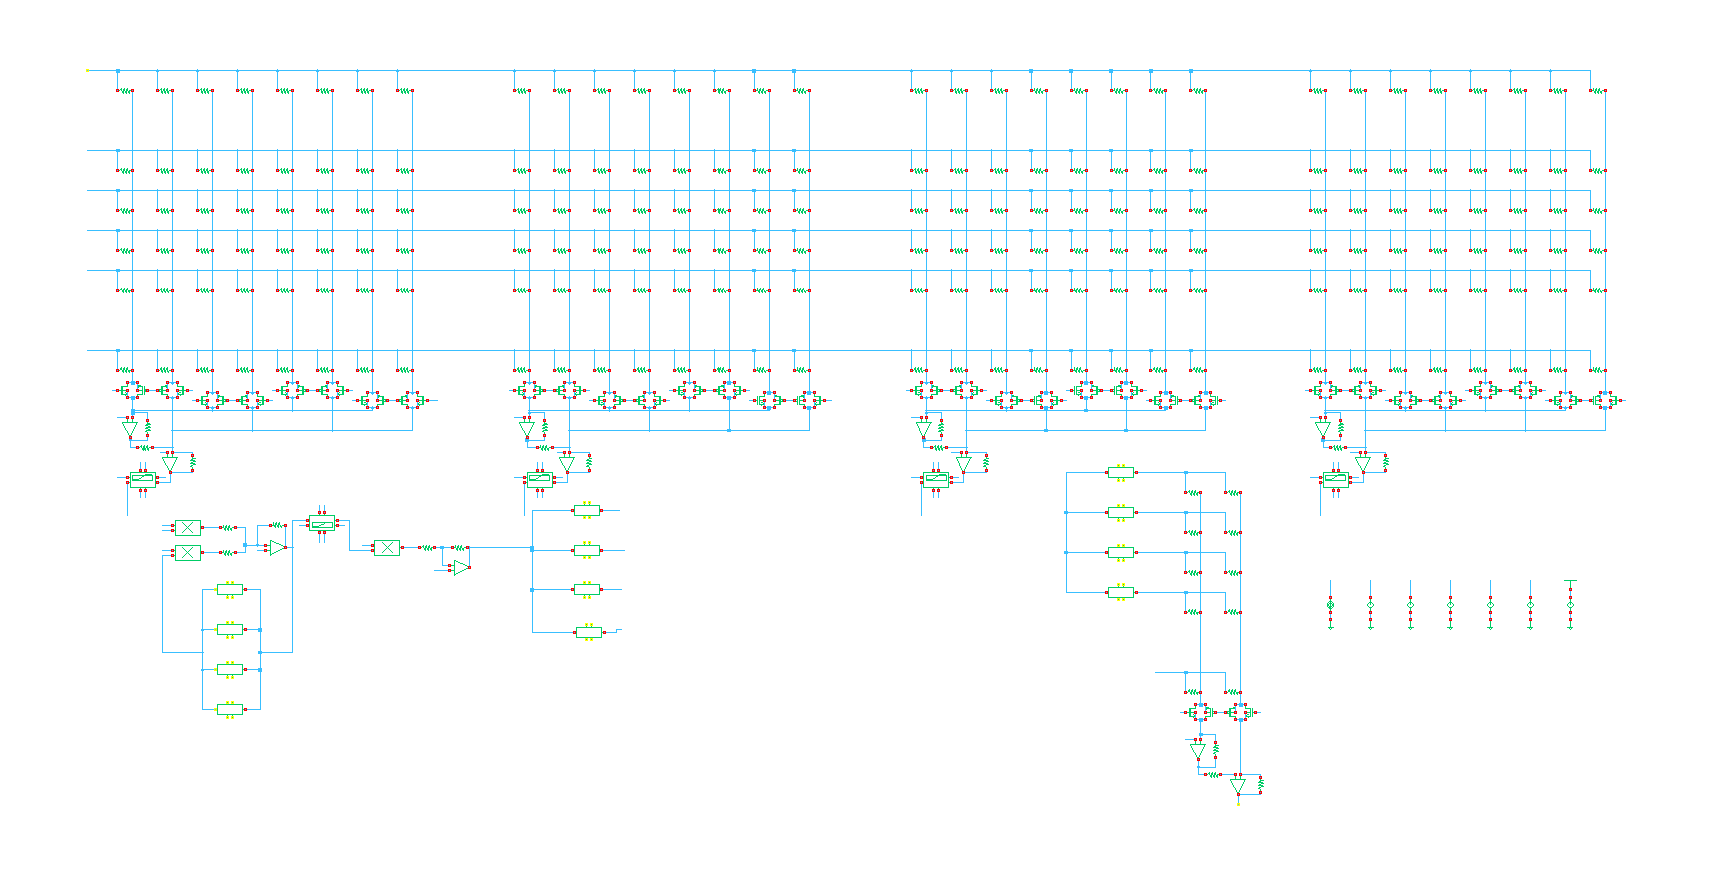
\includegraphics[height=0.5\textheight]{figures/LSTM-NP.png}
    \end{figure}
    Here the opamps and voltage multipliers are verilog-A models.
\end{frame}

% prepare question sigmoid 0 to 1


\section{Improvements to the model}
\begin{frame}{Serial vs parallel}
    The base paper uses serial computation.
    \begin{figure}
        \centering
        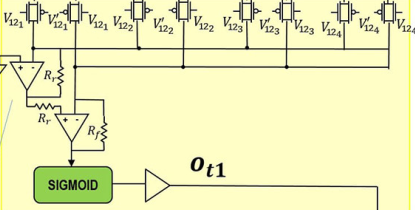
\includegraphics[height=0.5\textheight]{figures/parallel.png}
    \end{figure}
    It does so to save area on the chip.
\end{frame}
\begin{frame}{Serial vs parallel}
    That it is only useful for small LSTM networks.\\
    The area of the crossbar increase with $O(n_h^2)$.\\
    When the system is in parallel, the rest of the circuit is increasing with $O(n_h)$.\\
    When the system is in serial, the time it takes for one LSTM step increase with $O(n_h)$.\\
    At one point one LSTM step will become too long.\\
    We can fix that by either using a fully serialized system.\\
    The second would be to find out the optimal number of serial channel and use a mix of both.
\end{frame}

\section{Double OpAmps}
\begin{frame}{Double OpAmps}
    \begin{figure}
        \centering
        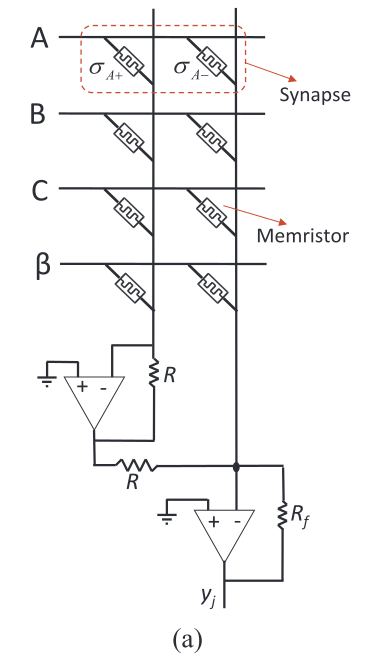
\includegraphics[height=0.35\textheight]{figures/doubleOpAmps.png}
    \end{figure}
    The final equation of this system is : $$y_j = R_f\cdot [A\cdot (\sigma_{A+}-\sigma_{A-})+ ... + \beta \cdot (\sigma_{\beta+}-\sigma_{\beta-})]$$
    That means that the weight is positive if $\sigma_+>\sigma_-$, and the inverse for the negative.
\end{frame}
\begin{frame}{Single OpAmp}
        There is a possibility of having only one OpAmp, that means having a threshold value to separate positive from negative. This also reduces the resolution of weights we can achieve.
\end{frame}

\section{Next step}
\begin{frame}{Matrix generation}
    I've been trying to generate an LSTM circuit from verilog, which doesn't work as we can't set the resistors values using that method. I'm going to use another netlisting tool (CDL, spice, other) to generate the system with preset resistances.
    Once I'll know how to do that, I'll be able to create a python script to create any LSTM wanted, the options can be changed very easily.
\end{frame}
\section{Question}
\begin{frame}{Normalized values}
    For the input the values have to be normalized. Usually using ranges like $[0.8,1]$(in V). Meaning that $1V$ is the maximum input value. The issue is that the sigmoid function goes from 0  to 1, but my design goes from $0.9V$ to $1V$, which with the conversion back to numbers goes from 0 to the max value.\\
    Have I missed somehting?
\end{frame}
\end{document}